\documentclass[brazil,times,12pt]{abnt}
\usepackage[T1]{fontenc}
\usepackage[utf8]{inputenc}
\usepackage{url}
\usepackage{graphicx}
% \usepackage[pdfborder={0 0 0}]{hyperref}
\makeatletter
\usepackage{babel}
\makeatother
\usepackage{listings}
\begin{document}

\autor{Pedro Paulo Vezzá Campos}

\titulo{Trabalho Prático 1: Interconexão de Computadores Usando Interface
RS-232}

\comentario{Trabalho apresentado para avaliação na disciplina INE5414, do
curso de Bacharelado em Ciências da Computação, turma 04208, da Universidade   
Federal de Santa Catarina, ministrada pelo professor Carlos Becker Westphall}

\instituicao{Departamento de Informática e Estatística \par Centro
Tecnológico \par Universidade Federal de Santa Catarina}

\local{Santa Catarina - SC, Brasil}

\data{\today}

\capa

\folhaderosto

% \tableofcontents
%\chapter{}
\section*{Objetivos}
	Para este primeiro trabalho prático foi proposto que fosse desenvolvido um
	software que possibilitasse a comunicação através da interface serial RS-232
	entre os dois microcomputadores, de tal forma que tudo que for digitado em um
	dos dois teclados apareça, simultaneamente, na tela de ambos microcomputadores.
	
	Neste realatório serão apresentados uma introdução ao protocolo RS-232, uma
	descrição das atividades realizadas para cumprir os requisitos impostos e por
	fim será apresentado o código fonte documentado do programa concluído.
	
\section*{Interface RS-232}
	RS-232 (Conhecido ainda por EIA RS-232C ou ITU V.24) é um protocolo de
	comunicação serial binária entre um Terminal de Dados, DTE e um Comunicador de
	Dados, DCE. \cite{wiki:rs232}

	Sua utilização original era conectara um teletipo (TTY) a um modem. Atualmente
	o RS-232 está na terceira revisão (RS-232C), publicadada em 1969 para
	adequar-se às características elétricas desses dispositivos. Posteriormente,
	ele foi utilizado com outros propósitos, tais como conectar equipamentos já
	existentes. Até os anos 90 o a porta RS-232 foi onipresente nos IBM-PCs sendo a
	maneira padrão de conectar um modem a um PC.
	
	Apesar de ter sido substituída em computadores modernos por barramentos mais
	velozes e compactos, tais como o USB e o Firewire, o RS-232 ainda possui grande
	importância como conexão para manutenção de equipamentos eletrônicos como
	televisões, decodificadores, no-breaks, dentre outros. Ainda, é uma maneira
	simples de conectar dispositivos remotos, tais como sensores externos que
	transmitem dados em baixa taxa de transferência.
	
	\subsection*{Protocolo}
	No protocolo de comunicação RS-232 comumentemente os caracteres são enviados
	um a um através de uma comunicação assíncrona utilizando bits de start e stop.
	Nesse estilo de codificação há o uso de um bit de início, seguido por sete ou
	oito bits de dados, possivelmente um bit de paridade, e um, 1,5 ou dois bits de
	parada. Assim, normalmente são necessários $1 + 8 + 1 = 10$ bits para enviar um
	único caractere. Portanto a relação entre dados úteis e dados transmitidos é de
	$7/10 = 0,7$. O padrão define os níveis elétricos correspondentes aos níveis
	lógicos um e zero, a velocidade de transmissão padrão e os tipos de
	conectores.\cite{strangio:rs232-standard}
	
	O padrão especifica 20 diferentes sinais de conexão, e um conector com formato
	de ``D'' (fig. \ref{fig:de9}) é comumente usado. São utilizados conectores
	machos e fêmeas - geralmente os conectores dos cabos são machos e os
	conectores de dispositivos são fêmeas - e estão disponíveis adaptadores m-m e
	f-f. Há também os chamados "null modems", que removem a necessidade de um modem
	interligando os dois terminais ao realizar uma ligação cruzada no cabeamento.
	Para a realização do trabalho prático foi utilizado um null modem, como será
	explicado adiante.
	
	\begin{figure}[htp]
	\begin{center}
		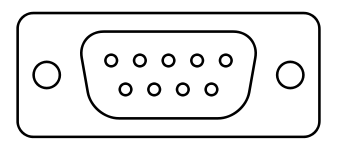
\includegraphics[width=70mm]{imagens/DE9.png}
		\caption[Diagrama de um conector DE9]{Diagrama de um conector DE9}
		\label{fig:de9}
	\end{center}
	\end{figure}
	
	O RS-232 é recomendado para conexões curtas (quinze metros ou menos) devido à
	grande capacitância gerada por cabos comuns de maior extensão. Os sinais variam
	de 3 a 15 volts positivos ou negativos, valores próximos de zero não são
	sinais válidos. O nível lógico um é definido por ser voltagem negativa, a
	condição de sinal é chamada "marca" e tem significado funcional de OFF
	(desligado). O nível lógico zero é positivo, a condição de sinal é chamda
	"espaço", e a função é ON (ligado). Níveis de sinal +-5, +-10, +- 12 e +-15
	são vistos comumente, dependendo da fonte elétrica
	disponível.\cite{strangio:rs232-standard}
	
	Três são os tipos de sinais nesses fios: terra, transmissão/recepção e
	"handshake". A tabela \ref{tab:de9} (obtida de \cite{anton:rs232-pinout})
	descreve de forma detalhada a função de cada um desses pinos:

	\begin{table}[h]
	\begin{center}
	\begin{tabular}{|c|c|c|c|}
		Pino & Sinal & In/Out & Descrição \\
		1 & DCD & In  & Data Carrier Detect \\
		2 & RxD & In  & Receive Data \\
		3 & TxD & Out & Transmit Data \\
		4 & DTR & Out & Data Terminal Ready \\
		5 & GND &  -  & Ground \\
		6 & DSR & In  & Data Set Ready \\
		7 & RTS & Out & Request to Send \\
		8 & CTS & In  & Clear to Send \\
		9 & RI  & In  & Ring Indicator
	\end{tabular}
	\end{center}
	\caption{Pinos do conector DE-9}
	\label{tab:de9}
	\end{table}
	
	O sinal de terra tem a função de aterrar as outras conexões e é necessário
	para identificar o 0V. Se os equipamentos estiverem muito longe, o terra 
	poderá mostrar-se diferente em cada uma das pontas do cabo, podendo gerar
	falhas na comunicação. Em conectores de 25 pinos, o pino 7 geralmente é o
	terra (pino 1 e terra do chassis são raramente usados). Neste mesmo conector,
	os pinos 2 e 3 são os pinos de transmissão e recepção, um dispositivo deve
	enviar no 2 e receber no 3; o outro deve ser o contrário (se não, essa
	inversão deve ser feita no fim do cabo, como num cabo para null modem, também
	chamado de crossover).
	
	Há várias configurações de software para conexões seriais. As mais comuns são
	velocidade e bits de paridade e parada. A velocidade é a quantidade de bits
	por segundo transmitida de um dispositivo para outro. Taxas comuns de
	transmissão são 300, 1200, 2400, 9600, 19200, etc. Tipicamente ambos os
	dispositivos devem estar configurados com a mesma velocidade, alguns
	dispositivos, porém, podem ser configurados para auto-detectar a velocidade. A
	paridade pode ser ímpar (todos os caracteres enviados terão um número ímpar de
	1's), par ou não estar ativada. Normalmente também pode-se escolher nos
	softwares de comunicação serial entre usar 1 ou 2 bits de parada. \cite{wiki:rs232}
	
\section*{Implementação do software de comunicação serial}
	\subsection*{Recursos utilizados}
	\begin{description}
	  \item[Windows XP] Versão 32 bits com SP3
	  \item[com0com] Software livre que implementa diversos null modens virtuais,
	  criando portas seriais virtuais utilizadas pelo programa criado.
	  \item[Python 2.7] Linguagem de programação adotada
	  \item[PySerial] Biblioteca de interfaceamento com portas seriais fornecidas
	  pelo sistema operacional.
	\end{description}

	\subsection*{Detalhamento do experimento}
	Diante da incapacidade de conectar fisicamente dois computadores por falta de
	portas DE-9 disponíveis e adaptadores DE-9/USB, foi adotada a opção de simular
	virtualmente uma porta serial. Para cumprir esse propósito foi adotado o
	com0com, um software livre exclusivo para Windows que atua como um null modem
	virtual criando portas seriais virtuais e interconectando-as. Através de uma
	interface gráfica (Fig \ref{fig:com0com}) intuitiva é possível alterar as configurações
	de pinagem além de outras opções que permitem simular situações do mundo real como taxas de
	transferência, ruído, etc.
	
	%\usepackage{graphics} is needed for \includegraphics
	\begin{figure}[htp]
	\begin{center}
  		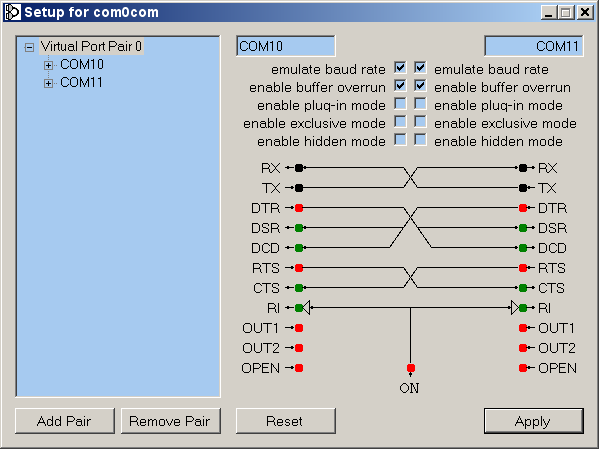
\includegraphics[width=120mm]{imagens/com0com-setup.PNG}
  		\caption[Interface do com0com]{Interface do com0com}
  	\label{fig:com0com}
	\end{center}
	\end{figure}
	
	Após a correta configuração do com0com e teste através do HyperTerminal,
	ferramenta embutida no Windows XP para comunicação entre dispositivos, 
	procedeu-se para a codificação do programa propriamente dito. Neste momento,
	Python apresentou-se como uma solução conveniente devido à facilidade de
	programação e rápida prototipação. Aliado ao Python há o PySerial, uma
	biblioteca de funções para interfaceamento entre programas Python e interfaces
	seriais. Seu funcionamento básico é através da criação de um objeto do tipo
	``Serial'' que conecta-se a uma porta serial especificada e obedecendo diversas
	configurações que abrangem desde taxa de transferência, paridade, número de
	bits de stop, tamanho do byte, etc. O envio de dados é através da função
	``write()'' que recebe como parâmetro uma string que é enviada ao terminal
	remoto, já o recebimento de dados ocorre através da função ``read()'' que
	retorna os caracteres armazenados no buffer da porta.
	
	O funcionamento básico do programa é o seguinte: 
	\begin{itemize}
  		\item Apresentação do programa ao usuário;
  		\item Pedido da porta desejada para conexão;
  		\item Pedido das configurações desejadas de taxa de transmissão, tamanho do
  		byte e número de bits de stop;
  		\item Início da conexão
  		\item Acionamento de duas ``threads'', ambas realizando polling, uma para o
  		recebimento de dados da porta e outra para o envio de dados
	\end{itemize}

	\subsection*{Código fonte}
	Abaixo segue o código fonte documentado do programa. Os pontos críticos do
	programa encontram-se nas threads, onde é realizado o polling de recebimento e
	envio de dados, ainda, a função ``iniciarConexao()'' é responsável por coletar
	as configurações desejadas e iniciar a conexão na porta escolhida.
	
	\lstset{language=Python,tabsize=4, numbers=left, numberstyle=\tiny}
	\lstinputlisting{src/TerminalSerial.py}
	\lstinputlisting{src/Getch.py}

\bibliographystyle{abnt-num}
\bibliography{bibliografia}
\end{document}